% !TEX root = main.tex

\section{Introduction}
\label{sec:intro}

The ability to grasp objects lies at the heart of robotic manipulation and therefore is fundamental to enabling robots to have complex physical interactions with their environment. 
Grasping a variety of unknown objects is challenging due to sensor and actuator uncertainty and uncertainty with respect to a new object's shape, mass distribution, texture properties, etc. 
Recently, deep neural networks have been used, with significant success, to address these challenges and enable robotic grasping. 

Within the context of this paper, we will make three assumptions with respect to our set-up. 
First, we will be grasping objects from a flat, clutter-free surface, such as an uncrowded table top. 
Second, we assume we have a method of generating \textit{grasp candidates}. 
Last, the robot has either an on-board camera or the environment the robot is operating in has a camera. 
Given an image of the scene captured by the camera, our goal is to evaluate which of these candidate grasps are likely to succeed. 
This creates a binary classification task, where the labels are grasp success and grasp failure. 

During execution, we can imagine that our robot with sample several grasps, execute a grasp that has been predicted to be successful via our classification method.  
Note that since attempting a grasp in a real world setting consumes time and can disrupt the environment, we would prefer to be cautious. 

For our data set we will use the Dexerity Network (DexNet) 2.0 data set, presented in~\cite{mahler2017dex}. 
The data set has 6.7 million grasps definitions, images and analytical grasp metrics, that we further detailed in \sref{sec:data_set}. 
The authors of the data set trained a Grasp Quality Convolutional Neural Network (GQ-CNN), seeen in \figref{fig:dexnet_network}, which achieved 85.7\% accuracy on their binary classification task.

While this is an impressive accuracy rate, we find that it is tied to the fact that nearly 80\% of the data is in the same class. 
When we re-balance the data distribution to have 50\% positive examples and negative examples, their same network achieves only 60\% accuracy. 

\begin{figure}[t!]
    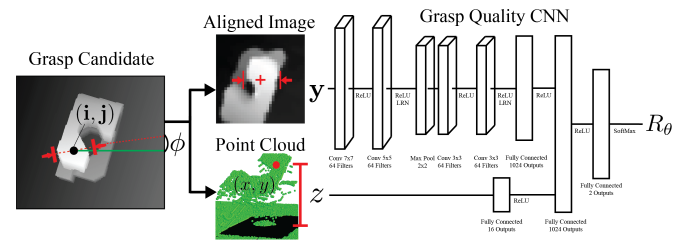
\includegraphics[width=0.99\columnwidth]{figs/dexnet.PNG}
\caption{This is a visualization the GQ-CNN (Grasp Quality Convolutional Neural Network) from \cite{mahler2017dex}. The network takes as input a depth image of the grasp and the distance of gripper to the object and output, after several layers, a prediction of grasp success.} \label{fig:dexnet_network}
\end{figure}

One fundamental assumption when learning is that the training sets and test sets are drawn from the same distribution. 
Maintaining this assumption, we found that this network (and others that we tried), had varying accuracy depending on the distribution. 
In this case, our results affirm the importance of considering the data distribution when evaluating learning algorithms. 

As mentioned, we explored several other architectures, with varying hyper parameters and normalization methods. 
However, we were unable to beat the accuracy rate achieved with the GQ-CNN. 

\textbf{We make the following contributions}:
\begin{enumerate}
    \item We explore the effect of the data set distribution on the accuracy of the model. Specifically, we modify the distribution of the training, validation and testing set and re-evaluate GQ-CNN.
		\item We adapt, train and evaluate three existing networks to our learning problem. 
		\item Using confusion matrices, we analyze the false positive and false negative ratio of our algorithms. From an algorithmic perspective, this helps us better examine the effect of varying data distributions. From a robotic perspective, this informs how efficient the robot might be when utilizing the results of the network. 
\end{enumerate}

We note that our comments with respect to data set distribution can only apply to our specific data set and the models we used. 
To make a more general claim we would need to more exhaustively test across different architectures and different data sets. 
Regardless, we found the effect of the data distribution to be an interesting artifact. 

With respect to the structure of the rest of the paper, we first review related work (\sref{sec:related_work}) and further detail the data set (\sref{sec:data_set}). 
Given our data set, we formally define our problem statement (\sref{sec:problem}) and then explore various data sets using the GQ-CNN (\sref{sec:balance}). 
We explore other architectures (\sref{sec:archs}) and conclude with a brief discussion (\sref{sec:discussion}). 
In particular, we discuss hypotheses on why were we unable to improve our accuracy rate and what makes this problem difficult. 

\begin{comment}

To accomplish the same task, we will be experimenting with new architectures, input formats, other modifications described in~\sref{sec:questions}.
Most of the recent machine learning papers in robotics present a problem, dataset and, usually, an optimized convolutional neural network with some architecture and input format. 
Our goal is to explore the process of finding that CNN and exploring the factors that effect performance. 
While our results will only be verified according to this data set, and therefore cannot be generalized to all CNNs, we hope to gain intution, understanding, and, hopefully, a higher accuracy. 
Having explored various components, we will optimize our final, best architecture. 
\end{comment}
